
% pnu_sampleEng.tex v1.0
% 본 양식은 서울대학교 전기컴퓨터공학부 학위논문 양식을 활용하여, 부산대학교의 양식에 맞춘 것입니다.
% https://ee.snu.ac.kr/community/notice/academic?bm=v&bbsidx=48811

% 논문작성을 위해서 한글패키지가 설치되어 있어야 합니다.
% MikTeX 을 사용할 것을 권장하며, MikTeX의 설치 및 한글 패키지와 관련된 사항은
% KTUG 한글 TeX 사용자 그룹 http://www.ktug.or.kr을 참조하시길 바랍니다.

% pnuthesis.cls file을 사용합니다.
% 박사의 경우 \documentclass[doctor]{pnuthesis} (default)
% 석사의 경우 \documentclass[master]{pnuthesis} 로 변경하면 됩니다.
% pnuthesis.cls file명이 바뀔경우에는 {pnuthesis} 대신에 {바뀐 file명}을 넣으면 됩니다.
% 주어진 .cls file의 내용을 변경하는 것은 규격에 어긋난 결과를 낼 수 있습니다.
%
% 주어진 .cls file은 부산대학교 논문 규격에 맞춰서 작성되어 있습니다.
% 변경 사항이 있을 경우, 적용하시길 바랍니다.

% 본 양식은 부산대학교 대학원에서 공식적으로 갱신하는 양식이 아닙니다.
% 활용에 따른 책임은 사용자에 있습니다.
% 조판 후 작성 된 것이 *규정에 맞는지* 꼭 확인하세요.

% 석사는 master, 박사는 doctor
% 영문은 english, 국문은 korean
\documentclass[doctor, english]{pnuthesis}

% UsePackages
\usepackage{lineno}
\usepackage{lipsum}

% 논문 작성을 위한 사전 준비과정
% 논문제목 (국문, 영문), 저자, 제출일, 심사일, 졸업일의 정보를 넣습니다.

% 논문제목을 넣습니다.
% 필히 한글제목과 영문제목 모두 넣어야 합니다.
\title[korean]{목탁의 물리적 요소와 발생하는 소리의 물리적 관계에 대한 연구}
\title[english]{A Study on the physical relationship between the Physical Properties of Wooden Gong and Sound Generated.}

% 저자 정보를 넣습니다.
% 국문성명, 영문성명 모두 넣어야 하며, 특히 국문성명의 경우는 글자사이에 space가 있는 것과 없는 것
% 두 가지 모두를 집어넣어줘야 합니다.
\author[korean]{박 보 검}
\author[english]{Eunwoo Cha}
\author[nospace]{박보검}

% 지도교수님의 성함을 국문 (영문 논문일 경우 영어로) 넣습니다.
\adviser[korean]{최 인 혁}
\adviser[english]{In-hyuk Choi}
\adviser[nospace]{최인혁}

% 논문 제출일, 논문 심사일을 한글(영문 논문일 경우 영어)로 넣습니다.
\examinationdate[korean]{2021년 11월 18일}
\examinationdate[english]{18, November, 2021}

% 졸업일을 영문식, 한글식 두 가지 방법 모두 넣습니다.
\gradyear[korean]{2022년 2월}
\gradyear[english]{FEBRUARY 2022}


\abstracts[korean]{
	국가안전보장에 관련되는 대외정책·군사정책과 국내정책의 수립에 관하여 국무회의의 심의에 앞서 대통령의 자문에 응하기 위하여 국가안전보장회의를 둔다. 모든 국민은 종교의 자유를 가진다. 대통령은 국가의 원수이며, 외국에 대하여 국가를 대표한다. 국무총리는 국무위원의 해임을 대통령에게 건의할 수 있다. 헌법재판소의 장은 국회의 동의를 얻어 재판관중에서 대통령이 임명한다. 타인의 범죄행위로 인하여 생명·신체에 대한 피해를 받은 국민은 법률이 정하는 바에 의하여 국가로부터 구조를 받을 수 있다. 국무총리·국무위원 또는 정부위원은 국회나 그 위원회에 출석하여 국정처리상황을 보고하거나 의견을 진술하고 질문에 응답할 수 있다.
}
\abstracts[english]{
	\lipsum[1]
}
%

% 문서의 시작
%
% 위의 정보들을 빠짐없이 채워넣고 document를 시작하면
% 외표지, 내표지(외표지와 동일), 인준지가 자동으로 생성됩니다.

% \linenumbers

\begin{document}
\renewcommand{\baselinestretch}{1.5}    % 본문의 줄간격 조정, 고치거나 삭제하지 마십시오.
\selectfont                             %

\changepage{5mm}{}{}{}{}{}{}{}{-5mm}    %%페이지 여백 재설정. 절대 고치거나 삭제하지 마십시오.
\makelists   %목차를 자동생성합니다.


% 본문의 시작
% chapter, section의 추가,변경등 모두를 자유롭게 할 수 있습니다.

\chapter{Lorem Ipsum Dolor Sit Amet}
\lipsum[1]
\section{Consectetur Adipiscing Elit}
\lipsum[2-3]
\begin{equation}
	y = \frac{-b \pm \sqrt{b^2-4ac}}{2a}
\end{equation}
\lipsum[11]
\subsection{Vestibulum Ut}
\lipsum[4]
\begin{figure}
	\centering
	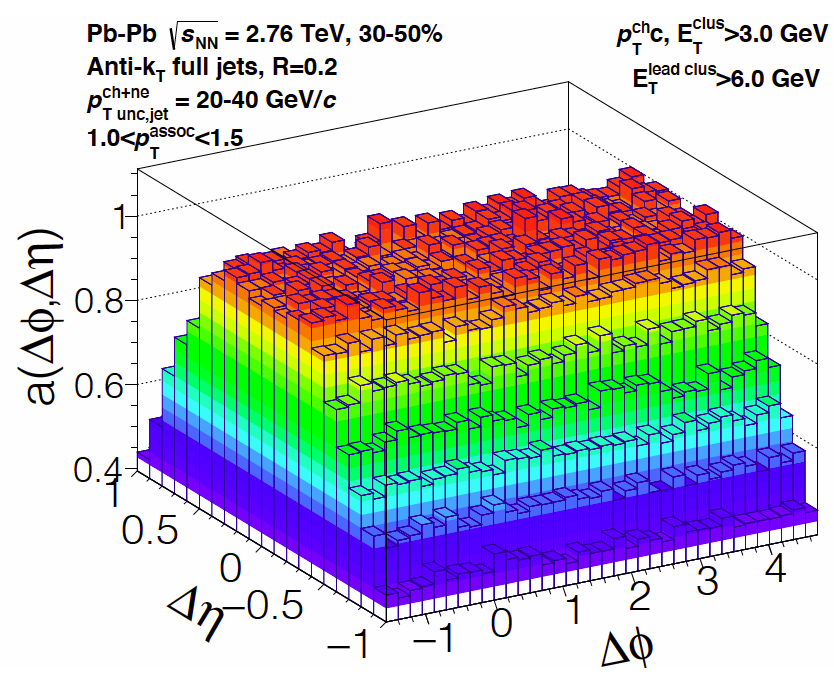
\includegraphics[width=0.7\textwidth]{figure/samplefig1.png}
	\caption{A sample figure to show}
\end{figure}
\lipsum[15]
\subsubsection{Un Hac Habitasse}
\lipsum[5]
\subsubsection{Morbi Vel Justo Vitae Lacus Rincidunt Ultrices}
\lipsum[6]
\subsection{Vestibulum Ut}
\lipsum[7]

\chapter{Sed Commodo Posuere Ped}
\lipsum[8-9]
\begin{figure}[!h]
	\centering
	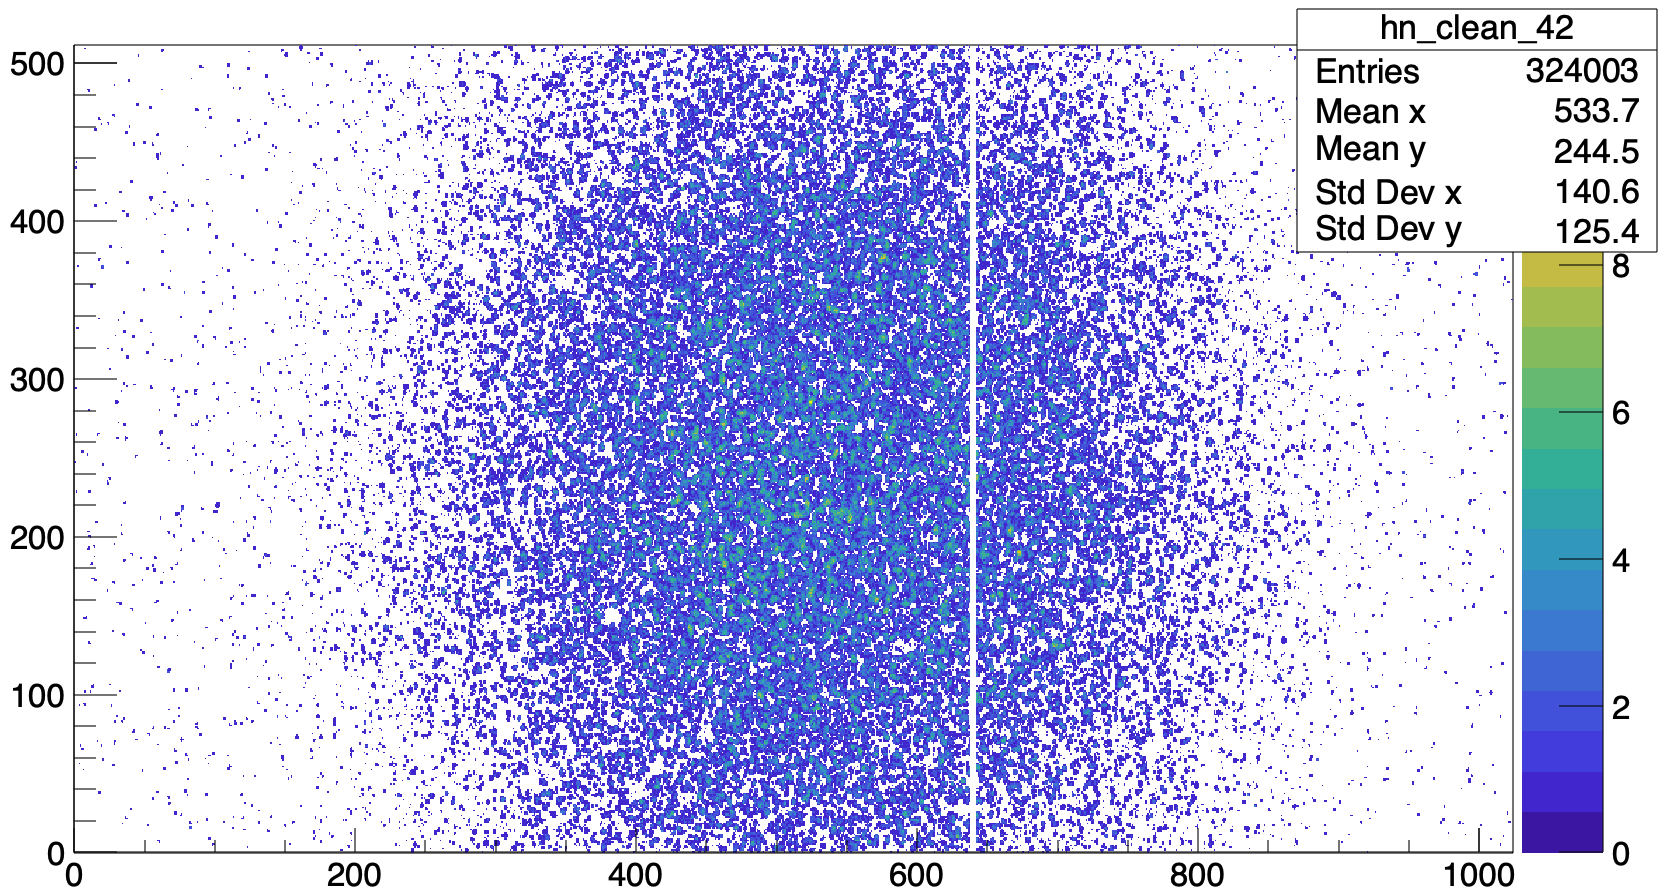
\includegraphics[width=0.7\textwidth]{figure/samplefig2.png}
	\caption{A 2nd figure to show}
\end{figure}
\lipsum[9-10]

%
% 참고문헌
%

\begin{thebibliography}{00}
	\bibitem{item1} Reference 1
	\bibitem{item2} Reference 2
	\bibitem{item3} Reference 3
\end{thebibliography}


\appendix
\chapter{Pellentesque Tristique Sodales Est}
\lipsum[12-14]

\pagebreak
\acknowledgement %감사의 글을 작성하지 않을경우 삭제가능

\lipsum[1-7]

\end{document}